\chapter{Implementation}

\section{Review of design diagrams}
    \subsection{Entities diagrams}
    \subsection{Interfaces diagrams}
    \subsection{Abstract factory to generate the questions}
    Due to maintenance reasons I opted to use this pattern to generate the questions. Imagine that, in the future, I want to add a new type of test. \\
    I should change all the logic in order to create just the questions for this test. \\
    As every question needs the same arguments in order to be created, just by using this pattern I would need to add a new question and factory. 
        \newpage
        \begin{figure}[H]
            \centering
                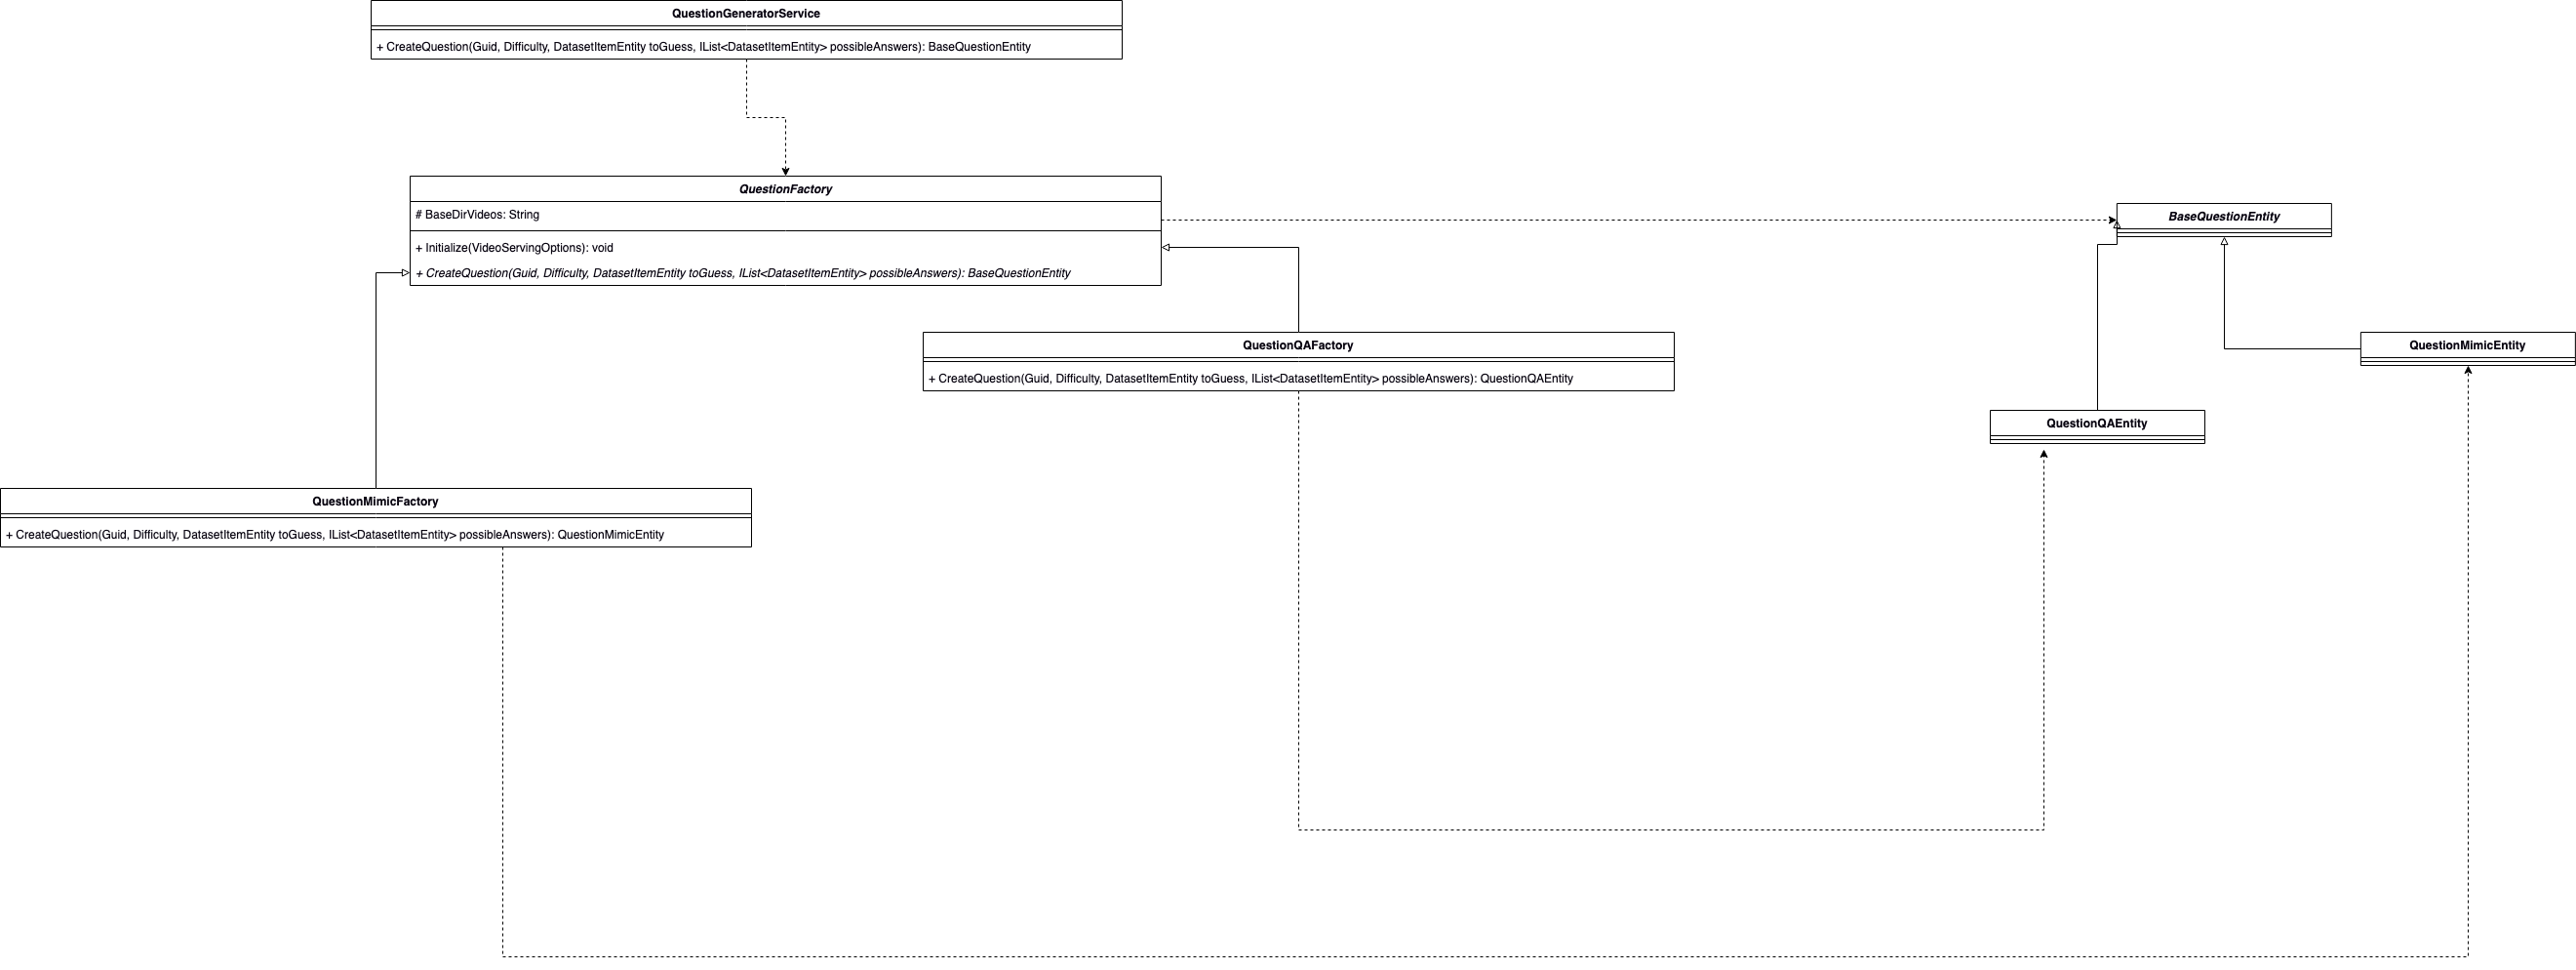
\includegraphics[angle=90, width=\textwidth, height=\textheight]{assets/diagrams/abstractfactory.png}
            \caption{Abstract factory}
            \label{fig:implementation_af}
        \end{figure}
\section{Sequence diagram, use case: \textit{Get a test}}
\section{Sequence diagram, use case: \textit{Delete a test}}
\section{Backend code documentation}
    \subsection{Architecture}
        \subsubsection{From MVC to Onion Architecture}
        \textbf{Model View Controller} (MVC) is the most commonly used web application architecture. It solves the separation of concern as there is a separation between \textit{View} (in this particular case the HTTP API responses), the \textit{Controller} (on which the business logic is added) and the \textit{Model} (it includes the database access).

        As we can see, we reach loose coupling, but tight coupling is still present. This is because classes are still dependent on concrete dependencies. \\

        \begin{figure}[H]
            \centering
                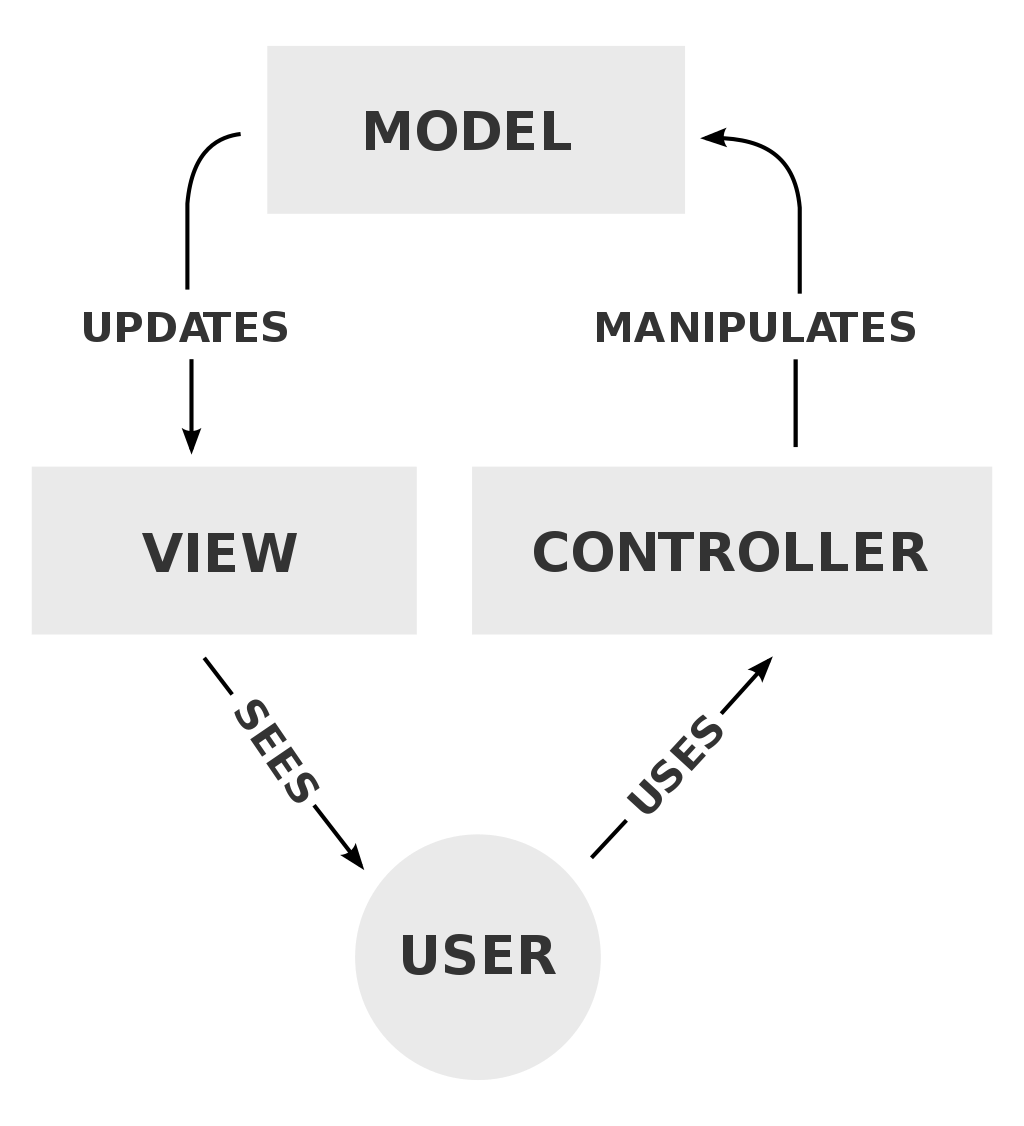
\includegraphics[width=0.5\textwidth]{assets/mvc.png}
            \caption{MVC \cite{MVC}}
            \label{fig:implementation_mvc}
        \end{figure}

        The \textbf{Onion Architecture} is very similar to \textit{MVC} because it keeps the separation of concerns but it solves the issue of tight coupling.

        \paragraph \textbf{How Onion architecture solves tight coupling?} \\
        It is based on Dependency Inversion Principle. All layers communicate with each other using interfaces. Concrete implementations are resolved on runtime. \\

        Layers are built on interfaces. This is also very convenient for testing purposes, due to the ease of exchanging a layer for a mock or another implementation object. \\
        The layers can change, but the idea is that all layers are towards to center, where the Core of the application is. It represents the business and behavior objects. \\

        \begin{figure}[H]
            \centering
                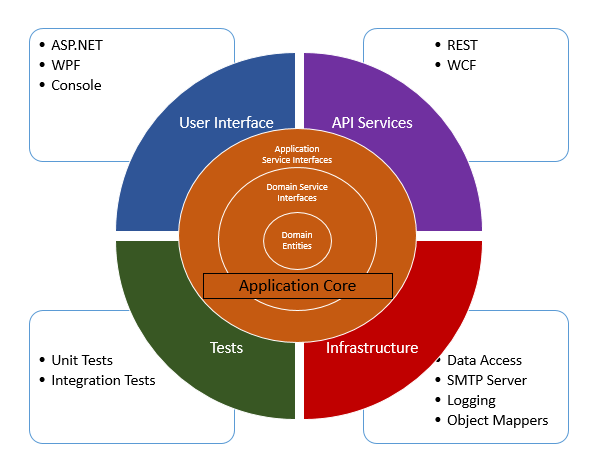
\includegraphics[width=\textwidth]{assets/onion.png}
            \caption{MVC \cite{OnionArchitecture}}
            \label{fig:implementation_onion}
        \end{figure}

        \subsubsection{How to orgnanize the project}
        \begin{itemize}
            \item Test: it is used for testing purposes.
                \begin{itemize}
                    \item References: all other layers.
                    \item Dependencies: xUnit.
                \end{itemize}
            \item Api: it is similar to view layer. It is the layer that will allow a client to interact with the application.
                \begin{itemize}
                   \item Reponsabilities (as directories):
                        \begin{itemize}
                            \item Controllers: define all the endpoints of the application and call the correct services on each method.
                            \item Middleware: catch users' calls to the Api. It allow to have a global exception handling, authorization, authentication...
                            \item Properties: define the launch settings for the Http Server.
                        \end{itemize}
                    \item References: Core
                    \item Dependencies:
                        \begin{itemize}
                            \item Api Rest: Asp.Net Core 5.0
                            \item Documentation: Swagger
                        \end{itemize}
                \end{itemize}
            \item Core: it is the center part of the architecture. It contains the definition of all the entities of the application, both contracts for the Api communication with the clients and the entities, both model and data access entities. It also contains all the interfaces which are used to communicate between the Api layer and the Infraestructure (Other authors separate this into a new layer: service layer). This contains all the business logic and works with the data source.
                \begin{itemize} 
                    \item Responsabilities (as directories):
                        \begin{itemize}
                            \item Contracts: instead of sending and receiving the entities in the Api, a good approach is to use DTO (Data Transfer Objects). This way, the user don't need to send the Id before creating an entity, we can avoid to send properties that may be confidential such as passwords and we can retrieve just the needed information.
                            \item CustomEntities: definition of application entities, such as metadata to send information about pagination in the api, pagination entity, etc
                            \item Entities: definition of data access models.
                            \item Enums
                            \item Exceptions: definition of custom exceptions.
                            \item Extensions: helper functions to improve code readability.
                            \item Interfaces: interfaces for repositories and services of the app.
                            \item Options: implementation of options pattern.
                            \item QueryFilters: filters for get Api methods.
                            \item Services: implementation of services to control de data access.
                            \item ValidationAttributes: attributes to validate models.
                        \end{itemize}
                    \item References: None
                    \item Dependencies: None
                \end{itemize}
            \item Infraestructure: concrete implementations of all the services needed by the app to work.
                \begin{itemize}
                    \item Responsabilities (as directories):
                        \begin{itemize}
                            \item Data: definition of the context and migrations.
                            \item Extensions: initialize all the services and dependency injection container.
                            \item Factories: to implement abstract factory pattern to initialize the questions.
                            \item Filters: add flux to validate the model in the Api.
                            \item Mappings: to convert an entity to a contract and reverse.
                            \item Migrations: database creation and updates.
                            \item Repositories: implementation of repositories and unit of work pattern.
                            \item Services: implementation of services based on external implementations. For instance: service to hash a password, send an email, create a JWT...
                            \item Validators: validation rules for the API filters to validate the model. For instance: email should be valid, password should have 'x' length, date should be greater than 'x'...
                        \end{itemize}
                    \item References: Core
                    \item Dependencies:
                        \begin{itemize}
                            \item Mail client: MailKit
                            \item ORM: Entity Framework Core
                            \item Validations: Fluent Validation
                            \item Logging: Serilog
                            \item Authentication: JWT
                            \item Mappings: automapper
                        \end{itemize}
                \end{itemize}
        \end{itemize}

        \subsubsection{Dependency injection}
        As this is a big project, following good design principles and patterns is important for its correct development and later maintenance. \\

        As the \textbf{SOLID principles} dictate, avoid depending on concrete implementations is a good practice as the application and its services may change. \\
        Instead of using the concrete implementations we let this work for interfaces. This way, the code in the upper layers won't change if the concrete implementation does, as the method signatures won't change. \\

        In ASP.NET it is recommended to use a dependency injection container and inject the dependencies in the constructor \cite{DI}. This way, the dependency injection container will change the interfaces for the concrete implementations and they will be passed automatically to the constructor. Let's see an example. \\

        In the next fragment of code, we can see how to configure the dependency injection container. This configuration corresponds to the \textit{Setup} class of the application. More concretely, it corresponds to the \textit{ConfigureServices} method, which receives an object that fits the \textit{IServicesCollection's interface} as an argument. \\
        This interface has the following methods to configure the dependency injection: \textit{AddTransient<Interface, Implementation>()}, \textit{AddSingleton<Interface, Implementation>()}, \textit{AddScoped<Interface, Implementation>()}. \\
        As we can notice, we can see a pattern: \textit{Add{LIFETIME}<{INTERFACE}, {IMPLEMENTATION}>()}. I'll talk about lifetime later on. \\

        The important thing here is that using these methods, the dependency injection container will know which object corresponds to every interface, so that we don't need to instanciate any object, the framework will do it for us. \\
        
        \lstinputlisting[language=CSharp, captionpos=t,
            caption={Dependency injection configuration}, 
            label={lst:impl_di_config}]
        {code/DependencyInjectionConfig.cs}
        

        In order to use these services, we can pass them through the constructor. We will have access only to the defined methods in the interface. The framework will automatically instanciate the object sending the correct object in the constructor. \\
        \lstinputlisting[language=CSharp, captionpos=t,
            caption={Dependency injection usage}, 
            label={lst:impl_di_usage}]
        {code/DependencyInjectionUsage.cs}
    

            \paragraph{Lifetime of an object}
            \begin{itemize}
                \item \textbf{Transient:} services are created each time they're requested. Best for lightweight, stateless services.
                \item \textbf{Scoped:} services are created once per client request (connection). Better option when you want to maintain state within a request.
                \item \textbf{Singleton:} services are created the first time they're requested.
            \end{itemize}

    \subsection{Defining environment variables and storing secrets}
    As the application grows, it is important to use environment variables. It is good to separate the app into multiple environments, so you can test, build and develop in separate contexts. \\
    Using environment variables you avoid to define global constants in the code, so you can change the behaviour of the application without compiling the whole app. It is also a good practice because you separate it \\
    correctly. \\
    
    But, when you think of storing all the configuration globals of the application you can get into a trap. You can define private information in these files, but this information should not be visible \\
    to all members in the team, it should not be uploaded into repositories and it should be encrypted. \\

    In this subsection, we'll see how the \textit{options pattern} resolves a way to manage all these fields. Also, we'll see how to store this secret information in a development environment and what to use in production. \\

        \subsubsection{Options pattern}
        In the next fragment of code we can see an usage of this pattern. First, I define the options themselves. For instance, I defined options to configure the pagination. Another examples of options could be the neccessary information to build an \\
        email client, such as username, client id, password or secret... \\
        
        After defining the structure of the options, we should tell the framework how and from where get the options. In this case, I defined the options in a JSON file to configure the app called \textit{appsettings.json}. \\
        Other options are defined in the secrets or could be defined in other environments, even on cloud. This way you can hide your secrets and avoid uploading these to repositories or to encrypt the secrets. \\

        Finally, to use the secrets you just need to resolve the interface. This will be done automatically using dependency injection containers in ASP.NET.
            \lstinputlisting[language=CSharp, captionpos=t,
                caption={Options}, 
                label={lst:impl_options}]
            {code/Options.cs}
        \subsubsection{Microsoft's development implementation: User secrets}
        See \href{https://docs.microsoft.com/en-us/aspnet/core/security/app-secrets?view=aspnetcore-5.0&tabs=windows}{here} for more information. Every piece of sensitive data is considered a secret. In order to store them in a safer way, we can use the \textit{Secret Manager Tool} provided by \textit{Microsoft}. \\
        The values are stored in a JSON file in the local machine. Due to this, it is not safe in a production environment as it is not encrypted. \\
        To make easier this task, I created the structure of all the secrets to configure in the app. This is the next code fragment. After modifying the JSON file with the correct information and just typing the commands in the next code fragment all the user secrets in the app will be correctly configured. \\

        \lstinputlisting[escapechar=+, language=json, captionpos=t,
            caption={JSON containing the definition for the user secrets}, 
            label={lst:impl_user_secrets_input}]
        {code/secrets.json}

        \lstinputlisting[escapechar=+, language=bash, captionpos=t,
            caption={Init and configure user secrets}, 
            label={lst:impl_user_secrets}]
        {code/usersecrets.bash}

        \subsubsection{Moving into a production environment}
        For production cases, it is recommended to use other options that provide encrypted store of the secrets. A recommended way by Microsoft is \textbf{Azure Key Vault} \cite{AKV}

    \subsection{Using extension methods to clean startup method}
    As the services and the configuration grow in the application, the \textit{Startup} class becomes less maintenable. Also, it would be good to separate the configuration in multiple files, as the responsability is different and the reason of change. \\
    
    \lstinputlisting[escapechar=+, language=CSharp, captionpos=t,
        caption={Refactoring startup method}, 
        label={lst:impl_startup_refactor}]
    {code/StartupExtensions.cs}

    All code is moved to this extension class. Passing the \textit{this} keyword to a static method, you can add the method to the object definition. The rest of the arguments will be the new method's arguments. \\
    This way only this new class will change whenever a new service is added, so the repository will be cleaner. The services object is returned so that the methods can be chained.
    \lstinputlisting[language=CSharp, captionpos=t,
        caption={Service collection's extensions methods}, 
        label={lst:impl_startup_extensions_1}]
    {code/StartupExtensions1.cs}

    \subsection{Entity framework}
        \subsubsection{Code first}
        Following \textit{Donatas Kimutis}'s recommendations \cite{Kimutis}, I use this approach. Firstly, I define the classes and mappings in the code. Then, the databases are created from the code. All evolutions are made via migrations. \\
        If the work is from an existing database, there are tool for reversing engineering. \\

        To mark navigational properties, I use \textit{virtual} keyword. This also enables \textit{Lazy Loading}, so these entities are only loaded when used. \\

        In the next fragment of code we can see the \textbf{User entity}. A user has the following properties:
        \begin{itemize}
            \item Email
            \item Password
            \item ConfirmedEmail
            \item TokenPasswordRecovery (optional)
            \item TokenEmailConfirmation (optional)
            \item Tests (navigation property). A user can have 0 or multiple tests.
        \end{itemize}

        \lstinputlisting[language=CSharp, captionpos=t,
            caption={User entity model creation}, 
            label={lst:impl_userentity}]
        {code/Virtual.cs}

        \subsubsection{Entity}
            In order to use generic repositories and track the events in the objects that will be stored in the database I need to create a base class. This class will be \textit{abstract}, as won't be instanciated. 
            
            \lstinputlisting[language=CSharp, captionpos=t,
                caption={Entity class}, 
                label={lst:impl_entity}]
            {code/Entity.cs}
        \subsubsection{Automatically tracking entities through events}
        When an operation with the database is made, the \textit{Entity framework} tracks the entity.  
        In the constructor of the \textit{DatabaseContext} class, I set up two methods to do when two events are fired. See \href{https://docs.microsoft.com/en-us/dotnet/api/microsoft.entityframeworkcore.changetracking.changetracker?view=efcore-5.0}{here}. \\

        When the event \textbf{StateChanged} is fired, the method \textit{OnEntityStateChanged} will be executed. It will update the parameter \textit{ModifiedOn} from the \textit{Entity} if the tracked entity is being modified.
        When the event \textbf{Tracked} is fired, the method \textit{OnEntityTracked} will be executed. It will update the parameter \textit{CreatedOn} from the \textit{Entity} if the tracked entity has been created.

            \lstinputlisting[language=CSharp, captionpos=t,
                caption={Entity tracking}, 
                label={lst:impl_entity_tracking}]
            {code/EntityTracking.cs}
        
        \subsubsection{Repository pattern}
            For this section, I used a guide from Microsoft \cite{RepoAndUW}. \\
            It is intended to add an abstraction layer between the data access and the business logic layer. To implement the repository pattern, I need to create an interface and an implementation for every entity in the application. \\
            As some functions are common for these entities, I can create a generic repository. \\

            In the next code fragment, I define the generic interface for the repositories. Note that the generic type \textit{T} should inherit from the \textit{BaseEntity}.
            \lstinputlisting[language=CSharp, captionpos=t,
                caption={Interface for the generic repository}, 
                label={lst:impl_ibaserepository}]
            {code/IBaseRepository.cs}

        \subsubsection{Unit of work pattern}
            For this section, I used a guide from Microsoft \cite{RepoAndUW}. \\
            As the application grows, more entities and repositories appear. The \textit{unit of work pattern} makes the use of these repositories cleaner and it ensures that all repositories share a single database context. \\

            \begin{figure}[H]
                \centering
                    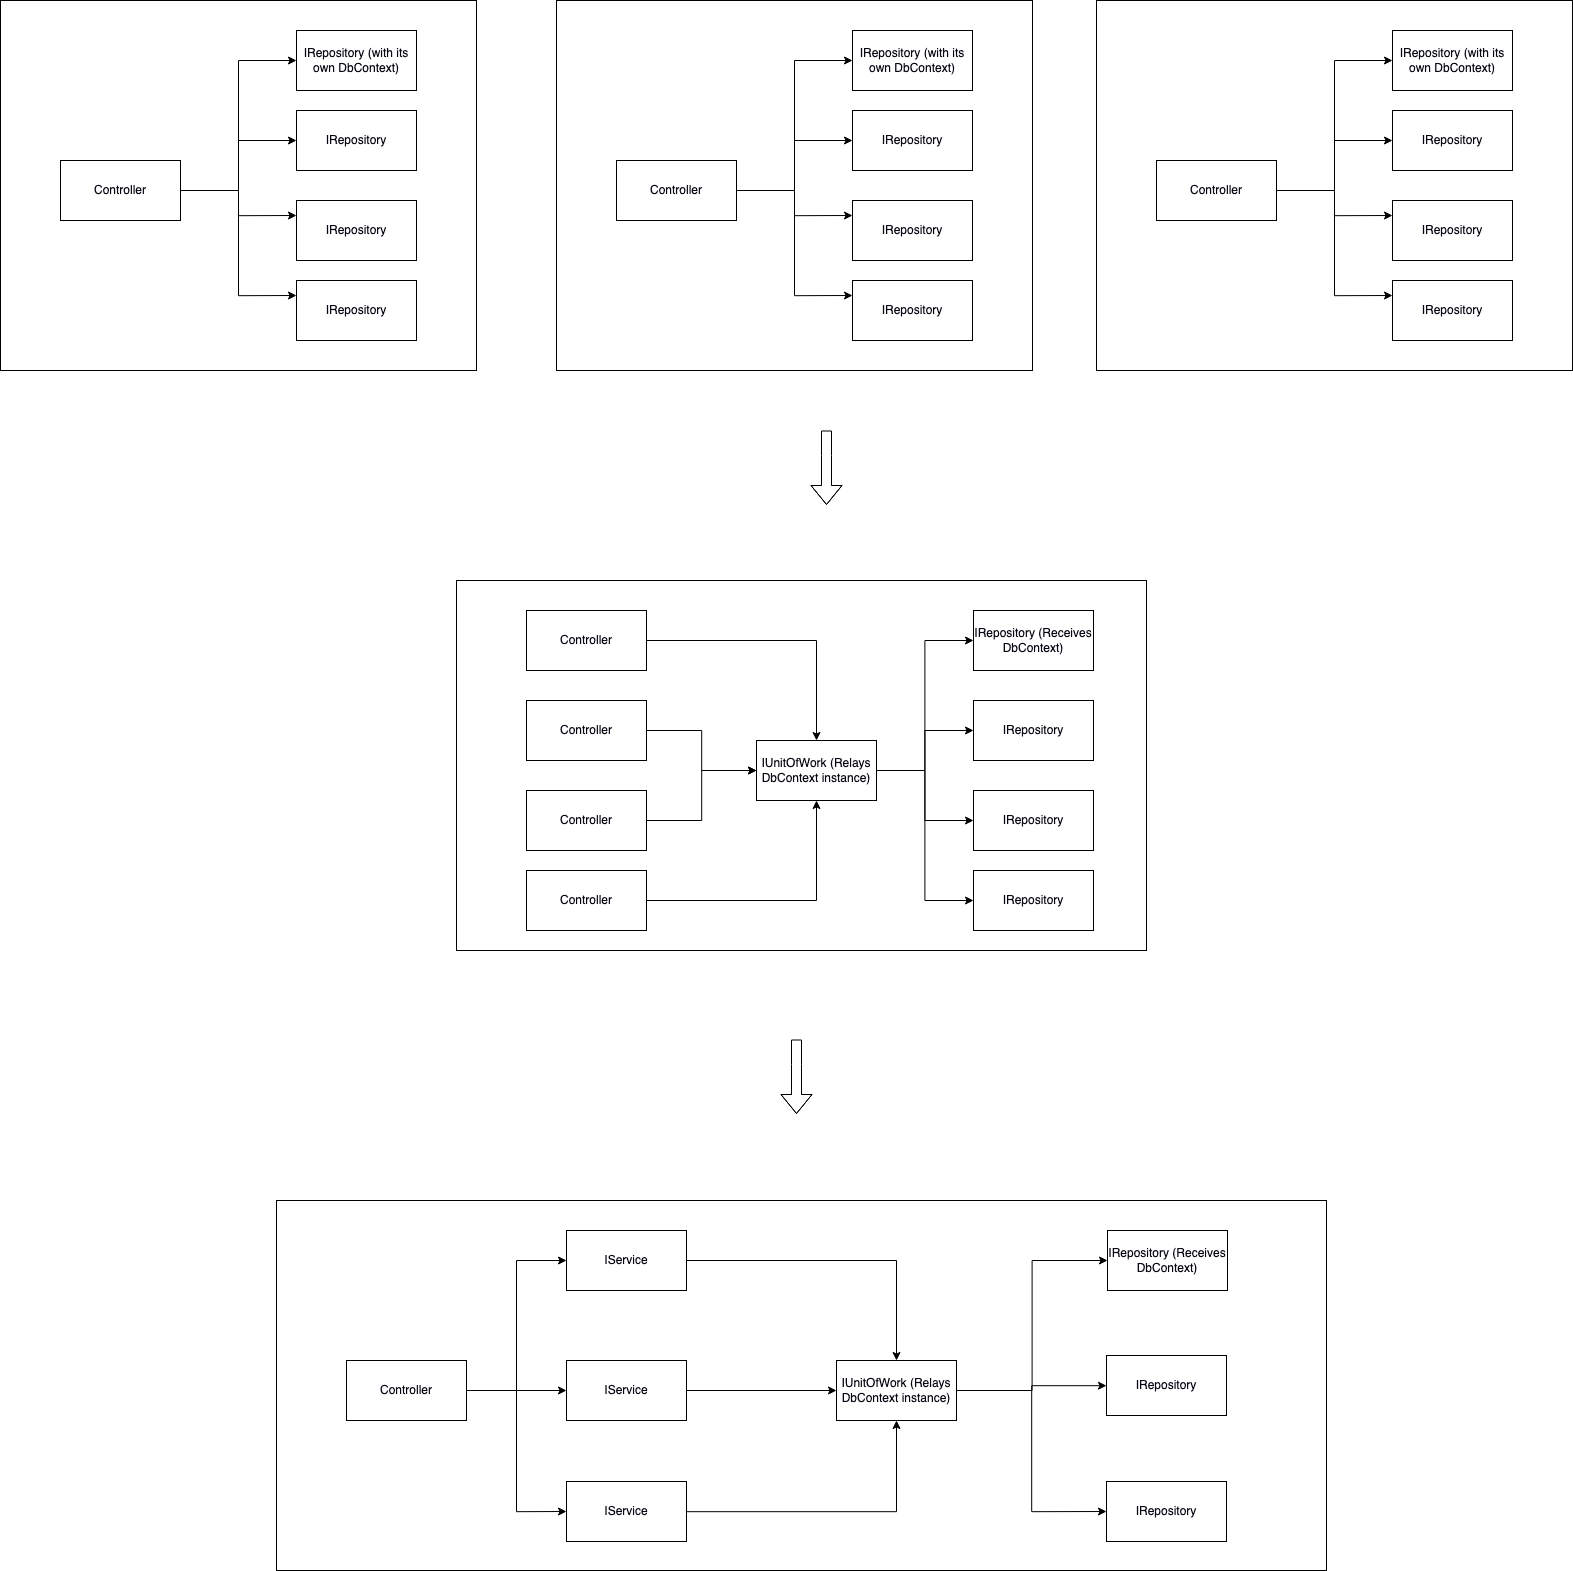
\includegraphics[width=0.9\textwidth]{assets/diagrams/unitofwork.png}
                \caption{Unit of Work}
                \label{fig:implementation_unit_work}
            \end{figure}
    
    \subsection{Error handling middleware}
    It is important to handle the errors of the application. Good reasons to do it could be to find errors in the code, send alerts if something has failed or stopped working, \\
    to avoid sending sensitive information to the client, etc. \\

    As we can see in the next code fragment, in the \textit{Startup} class I define the use of this middleware. \\
    The middleware capture the exceptions from the rest of middlewares and execution from the controllers. \\

    I catch all exceptions, although I do a separation: custom exceptions (\textit{BusinessExceptions} and \textit{ControllerExceptions}) and the rest. \\
    The custom exceptions are thrown by me, so I just send the error message to the client with a custom code. \\
    On the other hand, the rest of the exceptions are not handled by me. These could be network exceptions, from other dependencies such as the \textit{ORM}, etc. These exceptions are logged and \\
    the stack trace is sent to the client if the environment is set to \textit{Development}. \\
    \lstinputlisting[language=CSharp, captionpos=t,
        caption={Error handling middleware}, 
        label={lst:impl_ehm}]
    {code/ErrorHandlingMiddleware.cs}

        \subsubsection{Logger}
        All logs are saved in the \textit{Log} directory. The name of the file comes from the day. Every log entry contains the next information:
        \begin{itemize}
            \item Date and hour
            \item HTTP method from the request
            \item Route of the request
            \item Stack trace
        \end{itemize}
        \begin{figure}[H]
            \centering
                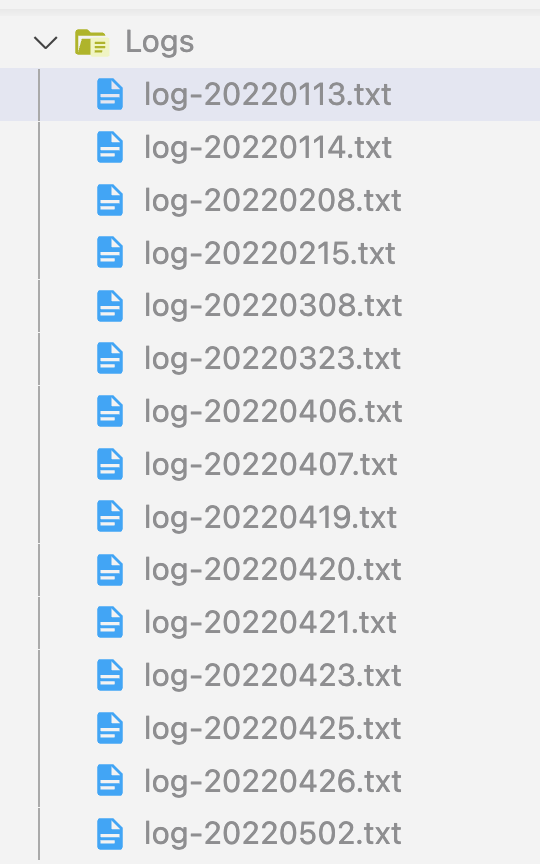
\includegraphics[width=0.3\textwidth]{assets/logs.png}
            \caption{Logs}
            \label{fig:implementation_logs}
        \end{figure}
        
    \subsection{Filters: automatic validation}
        \subsubsection{Using attributes}
        \subsubsection{Using validators}
    \subsection{Mapping}
        \subsubsection{Why using DTOs?}
        \subsubsection{Automapper}
    \subsection{Security}
        \subsubsection{Hashing passwords}
        \subsubsection{JWT tokens}
        \subsubsection{Configuring CORS}
    \subsection{Email service}
    \subsection{Pagination}
        \subsubsection{Why implementing pagination?}
        \subsubsection{How to implement pagination?}
    \subsection{Health check of the API}
    \subsection{Documenting the API with code using Swagger}
    \subsection{EXTRA: variant/invariant problem. How did I solve it?}
    \subsection{Middleware diagram}
    In the next page, I included a diagram that represents the flux that a request follows from the first moment it reaches the server until the servers replies to this request. \\

    The diagram contains all the middleware layers. The ones in yellow are the ones created/configured by me. The rest are simple configured by the framework. \\

    A good explanation of this diagram should explains every middleware layer. As this is a very detailed work and unneccessary, I'll just explain a bit of every layer:
    \begin{itemize}
        \item The uppest middleware layer is the \textit{Exception handler}. It is in charge of capturing the exceptions and reply correctly when something happens and log it.
        \item The \textit{Static files middleware} is in charge of give access to the filesystem. \\
        \item The \textit{CORS middleware} is in charge of configure the \textit{CORS} policy. \\
        \item The \textit{JWT middleware} is in charge of authorization and authentication. It checks the {JWT token} sent by the user in the request. 
        \item The \textit{Validation middleware} is in charge of validating the objects or fields sent in the {HTTP request}. This way, data sent incorrectly won't be processed. For instance, if the user asked for the tests done by him from tomorrow, this middleware would stop the flux as there can not be tests done from tomorrow. This query wouldn't go to the database. 
    \end{itemize}
        \newpage
        \begin{figure}[H]
            \centering
                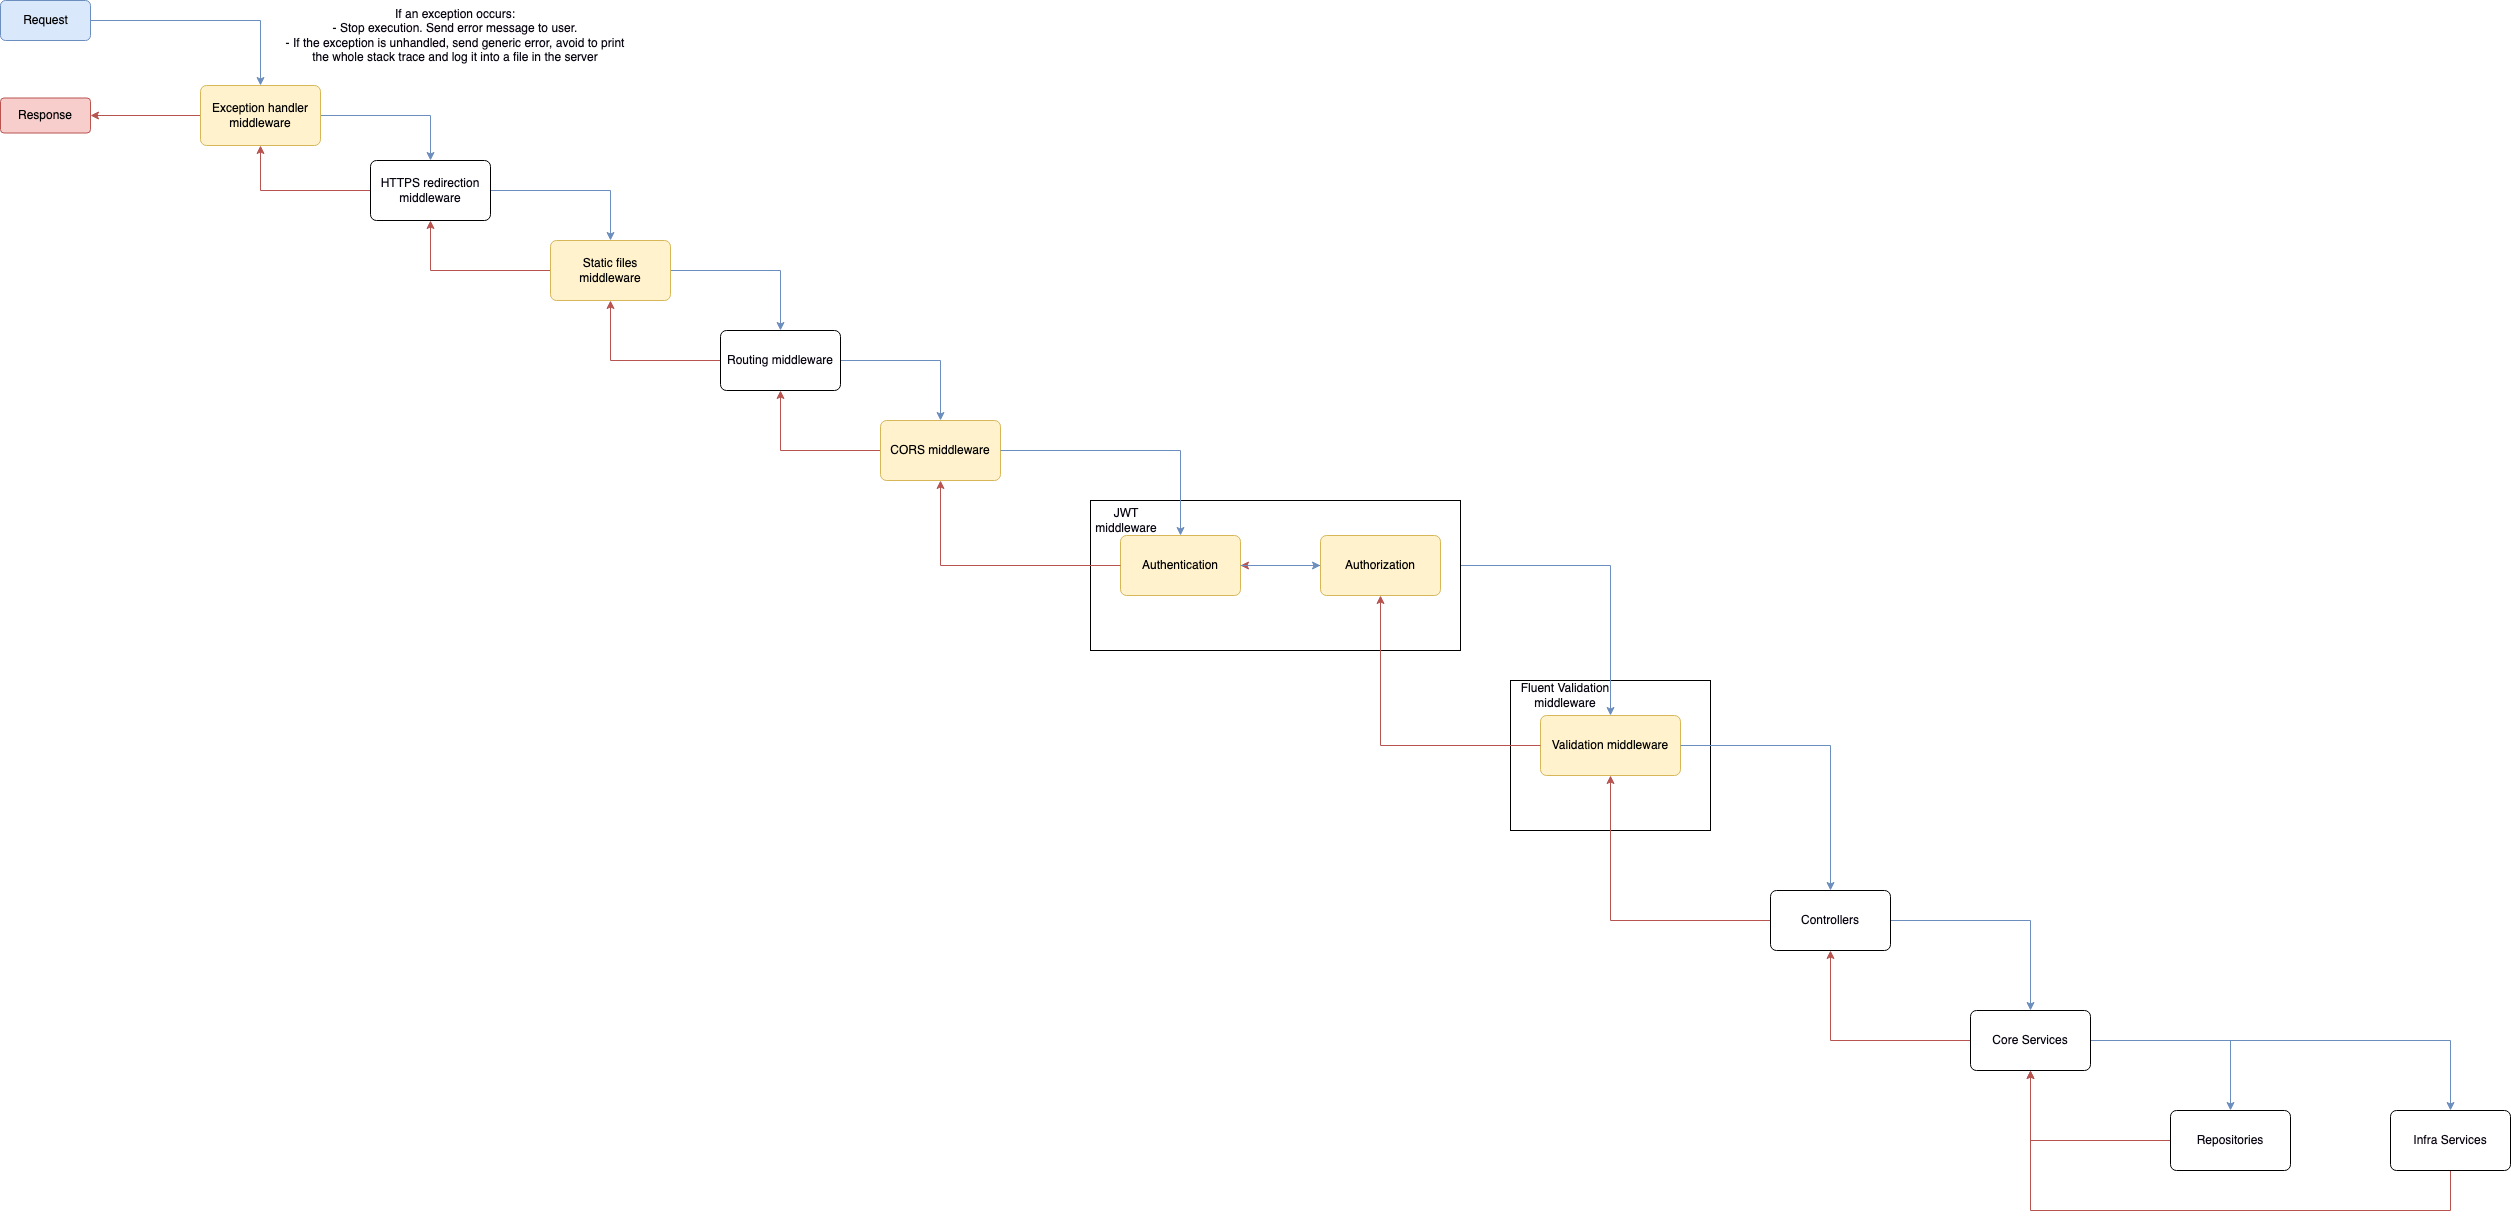
\includegraphics[angle=90, width=\textwidth, height=\textheight]{assets/diagrams/middleware.png}
            \caption{Middleware flux}
            \label{fig:implementation_middleware}
        \end{figure}

\section{Frontend code documentation}
    \subsection{Organization of the project}
    \subsection{Redux pattern}
    \subsection{Private VS public routes}
    \subsection{Intelligent forms using Formik}
        \subsubsection{Custom component to integrate Material UI and Formik}
    \subsection{Persisting the data}

\section{AI service code documentation}
    \subsection{API keys}
    \subsection{Protecting the API using JWT}
    \subsection{Validating the videos}
    \subsection{Initializing the model}
    \subsection{Executing the model}
        \subsection{Video transformations}
    \subsection{Example}
    
